\documentclass[]{article}
\usepackage{lmodern}
\usepackage{amssymb,amsmath}
\usepackage{ifxetex,ifluatex}
\usepackage{fixltx2e} % provides \textsubscript
\ifnum 0\ifxetex 1\fi\ifluatex 1\fi=0 % if pdftex
  \usepackage[T1]{fontenc}
  \usepackage[utf8]{inputenc}
\else % if luatex or xelatex
  \ifxetex
    \usepackage{mathspec}
  \else
    \usepackage{fontspec}
  \fi
  \defaultfontfeatures{Ligatures=TeX,Scale=MatchLowercase}
\fi
% use upquote if available, for straight quotes in verbatim environments
\IfFileExists{upquote.sty}{\usepackage{upquote}}{}
% use microtype if available
\IfFileExists{microtype.sty}{%
\usepackage{microtype}
\UseMicrotypeSet[protrusion]{basicmath} % disable protrusion for tt fonts
}{}
\usepackage[margin=1in]{geometry}
\usepackage{hyperref}
\hypersetup{unicode=true,
            pdfborder={0 0 0},
            breaklinks=true}
\urlstyle{same}  % don't use monospace font for urls
\usepackage{color}
\usepackage{fancyvrb}
\newcommand{\VerbBar}{|}
\newcommand{\VERB}{\Verb[commandchars=\\\{\}]}
\DefineVerbatimEnvironment{Highlighting}{Verbatim}{commandchars=\\\{\}}
% Add ',fontsize=\small' for more characters per line
\usepackage{framed}
\definecolor{shadecolor}{RGB}{248,248,248}
\newenvironment{Shaded}{\begin{snugshade}}{\end{snugshade}}
\newcommand{\KeywordTok}[1]{\textcolor[rgb]{0.13,0.29,0.53}{\textbf{#1}}}
\newcommand{\DataTypeTok}[1]{\textcolor[rgb]{0.13,0.29,0.53}{#1}}
\newcommand{\DecValTok}[1]{\textcolor[rgb]{0.00,0.00,0.81}{#1}}
\newcommand{\BaseNTok}[1]{\textcolor[rgb]{0.00,0.00,0.81}{#1}}
\newcommand{\FloatTok}[1]{\textcolor[rgb]{0.00,0.00,0.81}{#1}}
\newcommand{\ConstantTok}[1]{\textcolor[rgb]{0.00,0.00,0.00}{#1}}
\newcommand{\CharTok}[1]{\textcolor[rgb]{0.31,0.60,0.02}{#1}}
\newcommand{\SpecialCharTok}[1]{\textcolor[rgb]{0.00,0.00,0.00}{#1}}
\newcommand{\StringTok}[1]{\textcolor[rgb]{0.31,0.60,0.02}{#1}}
\newcommand{\VerbatimStringTok}[1]{\textcolor[rgb]{0.31,0.60,0.02}{#1}}
\newcommand{\SpecialStringTok}[1]{\textcolor[rgb]{0.31,0.60,0.02}{#1}}
\newcommand{\ImportTok}[1]{#1}
\newcommand{\CommentTok}[1]{\textcolor[rgb]{0.56,0.35,0.01}{\textit{#1}}}
\newcommand{\DocumentationTok}[1]{\textcolor[rgb]{0.56,0.35,0.01}{\textbf{\textit{#1}}}}
\newcommand{\AnnotationTok}[1]{\textcolor[rgb]{0.56,0.35,0.01}{\textbf{\textit{#1}}}}
\newcommand{\CommentVarTok}[1]{\textcolor[rgb]{0.56,0.35,0.01}{\textbf{\textit{#1}}}}
\newcommand{\OtherTok}[1]{\textcolor[rgb]{0.56,0.35,0.01}{#1}}
\newcommand{\FunctionTok}[1]{\textcolor[rgb]{0.00,0.00,0.00}{#1}}
\newcommand{\VariableTok}[1]{\textcolor[rgb]{0.00,0.00,0.00}{#1}}
\newcommand{\ControlFlowTok}[1]{\textcolor[rgb]{0.13,0.29,0.53}{\textbf{#1}}}
\newcommand{\OperatorTok}[1]{\textcolor[rgb]{0.81,0.36,0.00}{\textbf{#1}}}
\newcommand{\BuiltInTok}[1]{#1}
\newcommand{\ExtensionTok}[1]{#1}
\newcommand{\PreprocessorTok}[1]{\textcolor[rgb]{0.56,0.35,0.01}{\textit{#1}}}
\newcommand{\AttributeTok}[1]{\textcolor[rgb]{0.77,0.63,0.00}{#1}}
\newcommand{\RegionMarkerTok}[1]{#1}
\newcommand{\InformationTok}[1]{\textcolor[rgb]{0.56,0.35,0.01}{\textbf{\textit{#1}}}}
\newcommand{\WarningTok}[1]{\textcolor[rgb]{0.56,0.35,0.01}{\textbf{\textit{#1}}}}
\newcommand{\AlertTok}[1]{\textcolor[rgb]{0.94,0.16,0.16}{#1}}
\newcommand{\ErrorTok}[1]{\textcolor[rgb]{0.64,0.00,0.00}{\textbf{#1}}}
\newcommand{\NormalTok}[1]{#1}
\usepackage{graphicx,grffile}
\makeatletter
\def\maxwidth{\ifdim\Gin@nat@width>\linewidth\linewidth\else\Gin@nat@width\fi}
\def\maxheight{\ifdim\Gin@nat@height>\textheight\textheight\else\Gin@nat@height\fi}
\makeatother
% Scale images if necessary, so that they will not overflow the page
% margins by default, and it is still possible to overwrite the defaults
% using explicit options in \includegraphics[width, height, ...]{}
\setkeys{Gin}{width=\maxwidth,height=\maxheight,keepaspectratio}
\IfFileExists{parskip.sty}{%
\usepackage{parskip}
}{% else
\setlength{\parindent}{0pt}
\setlength{\parskip}{6pt plus 2pt minus 1pt}
}
\setlength{\emergencystretch}{3em}  % prevent overfull lines
\providecommand{\tightlist}{%
  \setlength{\itemsep}{0pt}\setlength{\parskip}{0pt}}
\setcounter{secnumdepth}{0}
% Redefines (sub)paragraphs to behave more like sections
\ifx\paragraph\undefined\else
\let\oldparagraph\paragraph
\renewcommand{\paragraph}[1]{\oldparagraph{#1}\mbox{}}
\fi
\ifx\subparagraph\undefined\else
\let\oldsubparagraph\subparagraph
\renewcommand{\subparagraph}[1]{\oldsubparagraph{#1}\mbox{}}
\fi

%%% Use protect on footnotes to avoid problems with footnotes in titles
\let\rmarkdownfootnote\footnote%
\def\footnote{\protect\rmarkdownfootnote}

%%% Change title format to be more compact
\usepackage{titling}

% Create subtitle command for use in maketitle
\newcommand{\subtitle}[1]{
  \posttitle{
    \begin{center}\large#1\end{center}
    }
}

\setlength{\droptitle}{-2em}

  \title{}
    \pretitle{\vspace{\droptitle}}
  \posttitle{}
    \author{}
    \preauthor{}\postauthor{}
    \date{}
    \predate{}\postdate{}
  

\begin{document}

\begin{quote}
\emph{For precept must be upon precept, precept upon precept; line upon line, line upon line; here a little, and there a little.}
--- Isaiah 28:10, King James Bible
\end{quote}

\doublespacing

\section{Introduction}\label{introduction}

As presented in the previous chapter, Marginal Mediation Analysis (MMA)
has the ability to simplify the interpretation of mediated effects in a
wide variety of situations, particularly in situations where an effect
size otherwise does not exist (e.g., indirect effects when the mediator
or outcome is categorical). In this chapter, methods fashioned to
develop MMA and evaluate its performance are discussed via three phases:

\begin{enumerate}
\def\labelenumi{\arabic{enumi}.}
\tightlist
\item
  Development of MMA
\item
  Monte Carlo Simulation Study of MMA
\item
  Application of MMA
\end{enumerate}

\noindent These phases were designed to provide the theory and the
software to perform MMA, assess the method's ability to accurately
estimate the underlying effects, develop the guidelines of its use in
finite samples, and apply it to real-world prevention data by
replicating a recent study {[}@Ford2012{]} that used a categorical
mediator and categorical outcomes. Below, each phase is described in
depth.

\section{Phase I: Development of Marginal Mediation
Analysis}\label{phase-i-development-of-marginal-mediation-analysis}

To be useful to public health, psychological, and prevention
researchers, the incorporation of average marginal effects within
mediation analysis must happen in two ways: in theory and in software.
This phase is focused on understanding the properties of MMA and on
developing the software necessary to perform it.

\subsection{Properties of MMA}\label{properties-of-mma}

Building on the mediation framework discussed by @Hayes2009 and by
Edwards and Lambert (2007), MMA was established on linear
regression---either ordinary least squares (OLS) for continuous
outcomes/mediators or maximum likelihood (via GLMs) for categorical
outcomes/mediators. In this framework, two or more regression equations
are combined to provide the overall mediation model as discussed in
Chapter 1. This method then adds a post-estimation step (Chapter 2) into
this mediation framework.

The form of the general marginal mediation model, including the
post-estimation step, were discussed in Chapter 3. Using this general
framework, various considerations were made in the development of the
method. First, an appropriate manner in which to integrate moderation
(interaction effects) into the framework is important. Because of the
work by Edwards and Lambert (2007), this included assessing the
\emph{reduced
form}\footnote{Reduced form refers to only having exogenous variables on the right-hand side of a regression equation (i.e., substituting the predictors of the mediators into the equation).}
of the models in addition to visualizations of the predicted values
across levels of the moderator. Second, it has been noted by
@mackinnon2008intro that in non-linear models the \(a \times b + c'\)
generally does not equal the \(c\) path as it does in linear models
(Chapter 11 in his book). To assess whether these are equal within MMA,
both a basic analysis and a Monte Carlo simulation (phase II) was used.

\subsection{Software Development}\label{software-development}

A major aspect of this first phase is the development of the software
for researchers to apply MMA. This software is provided via the R
statistical environment given R is free, widely used by researchers in
health and prevention, and extensions to the software via ``packages''
are efficiently disseminated through the Comprehensive R Archive Network
(CRAN). It consists of a number of functions to fit the model and assess
the model's fit while efficiently producing the paths and effects in
proper units.

Because of the flexibility of numerical derivation methods and the speed
improvements by Thomas Leeper (2017), numerical derivatives were used to
obtain the marginal effects for each observational unit. From here,
means of the marginal effects were calculated for each variable in the
model. To assess the model uncertainty, bootstrapping via the
\texttt{boot} R package was applied. This approach relies on repeated
resampling from the original sample \emph{with replacement}. In general,
this method does not rely on any distributional assumptions and works
well with asymmetric distributions (as is found in indirect effects).

The package applies the best practices for both computational speed and
user readability {[}@Wickham2015{]}, allowing other researchers to
extend the package more easily. Additionally, several built-in tests
will inform the functionality of the package before beginning Phase 2.
These tests were performed on Linux, Mac, and Windows platforms.
Finally, the package uses Git as the version control system. The
necessary functions were developed first so that the package tests and
simulations could begin. The usability of the package that is important
in the disseminated version were developed afterwards.

\section{Phase II: Monte Carlo Simulation Study of Marginal Mediation
Analysis}\label{phase-ii-monte-carlo-simulation-study-of-marginal-mediation-analysis}

The evaluation of MMA is an essential step in understanding its
properties and robustness and further assess the performance of the
software. The consistency of MMA, the statistical power at various
sample sizes, and the accuracy of the bootstrapped confidence intervals
were all tested via a Monte Carlo simulation study {[}@Paxton2001;
@Carsey2013{]}.

In the simulation, data were simulated to come from a population of
known parameters. A literature review of mediation analysis in
prevention work highlighted the appropriateness of the population
parameters chosen. The results of the simulation helped in the
development of the guidelines for using MMA in practice.

\subsection{Literature Review}\label{literature-review}

Before performing the Monte Carlo simulations, a review of the
literature is recommended {[}@Paxton2001{]}. This review focused on the
use of mediation analysis in prevention research where the analyses
contained categorical mediators and/or outcomes. This review included
all recent articles (2008 - 2017) found that clearly identified a
mediator or outcome that was categorical in nature. This search relied
on terms such as ``generalized linear models'', ``logistic'',
``dichotomous'', ``polytomous'', and ``count'' in conjunction with
``mediation analysis'' across the Scopus database.

\subsection{Simulations}\label{simulations}

Monte Carlo simulations, via the R statistical environment version
3.4.2, assessed the finite properties of MMA. Monte Carlo simulation was
selected due to its simplicity in generating informative results and its
high success in the literature {[}e.g., @Graham2007; @Nylund2007{]}.
Here, 500 data sets were simulated for each combination of experimental
conditions {[}@Paxton2001; @Carsey2013{]}. The data were simulated from
a known population with a researcher specified causal model (i.e., the
``population model''). The model consisted of either a binary mediator
(0 = ``No'', 1 = ``Yes'') or a count variable (Poisson distribution), a
continuous outcome, and a continuous predictor while also varying the
sample size and the effect sizes for a total of 90 unique combinations
of the conditions (see Table \ref{tab_conditions}).

The \(a\) path population model is defined below for when the mediator
is binary, where the \(Prob(M_{u} = 1)\) is a latent continuous variable
with a logistic relationship with the predictors and the \(\epsilon_i\)
is normally distributed with a mean of 0 and a standard deviation of 1.

\begin{equation}
log(\frac{Prob(M_{u} = 1)_{i}}{1 - Prob(M_{u} = 1)_{i}}) = a_0 + a_1 x + \epsilon_i
\end{equation}

\noindent The observed variable, \(M_{o}\), is defined as follows:

\begin{equation}
M_{o} = \begin{cases}
            0, & \text{if } Prob(M_u = 1) < .5, \\
            1, & \text{otherwise}.
         \end{cases}
\end{equation}

The \(a\) path population model for when the mediator is a count is
shown below where \(M_u\) is a latent continuous variable with an
exponential relationship with the predictors and the \(\epsilon_i\) is
normally distributed with a mean of 0 and a standard deviation of 1.

\begin{equation}
log(M_u) = a_0 + a_1 x + \epsilon_i
\end{equation}

\noindent The observed variable, \(M_{o}\), is defined as follows:

\begin{equation}
M_{o} = Po(\lambda = M_u)
\end{equation}

\noindent This creates an observed, count variable that has \(\lambda\)
values based on the latent mediator.

The \(b\) and \(c'\) paths population model is identical to Equation
\ref{equation_b} with only one predictor and a single binary, or count,
mediator, as shown below.

\begin{equation}
M_{i} = a_0 + a_1 x_1 + \epsilon_{mi}
\end{equation}\begin{equation}
Y_{i} = \beta_0 + b M_{i} + c^{'} x_{i} + \epsilon_{yi}
\end{equation}

\begin{Shaded}
\begin{Highlighting}[]
\KeywordTok{options}\NormalTok{(}\DataTypeTok{xtable.comment =} \OtherTok{FALSE}\NormalTok{)}
\KeywordTok{library}\NormalTok{(readr)}
\NormalTok{tab =}\StringTok{ }\KeywordTok{read_csv}\NormalTok{(}\StringTok{"C:/Users/User/Documents/DissertateGitUCU/Dissertate/ConditionsTable.csv"}\NormalTok{)}
\KeywordTok{names}\NormalTok{(tab) =}\StringTok{ }\KeywordTok{c}\NormalTok{(}\StringTok{"Independent Variables"}\NormalTok{, }\StringTok{"Conditions"}\NormalTok{)}
\NormalTok{tab[}\DecValTok{4}\NormalTok{,}\DecValTok{2}\NormalTok{] =}\StringTok{ }\KeywordTok{c}\NormalTok{(}\StringTok{".30"}\NormalTok{)}
\NormalTok{tab[}\DecValTok{7}\NormalTok{,}\DecValTok{2}\NormalTok{] =}\StringTok{ }\KeywordTok{c}\NormalTok{(}\StringTok{"90"}\NormalTok{)}
\NormalTok{tab[}\DecValTok{6}\NormalTok{,}\DecValTok{1}\NormalTok{] =}\StringTok{ }\NormalTok{tab[}\DecValTok{6}\NormalTok{,}\DecValTok{2}\NormalTok{] =}\StringTok{ " "}
\KeywordTok{library}\NormalTok{(xtable)}
\NormalTok{tabx =}\StringTok{ }\KeywordTok{xtable}\NormalTok{(tab[, }\DecValTok{1}\OperatorTok{:}\DecValTok{2}\NormalTok{], }
       \DataTypeTok{label =} \StringTok{"tab_conditions"}\NormalTok{, }
       \DataTypeTok{caption =} \StringTok{"The various experimental conditions of the Monte Carlo simulation study."}\NormalTok{,}
       \DataTypeTok{align =} \KeywordTok{c}\NormalTok{(}\StringTok{"l"}\NormalTok{, }\StringTok{"|l"}\NormalTok{, }\StringTok{"|c|"}\NormalTok{))}
\KeywordTok{print.xtable}\NormalTok{(tabx, }\DataTypeTok{include.rownames =} \OtherTok{FALSE}\NormalTok{, }\DataTypeTok{caption.placement =} \StringTok{"top"}\NormalTok{,}
             \DataTypeTok{table.placement =} \StringTok{"tb"}\NormalTok{)}
\end{Highlighting}
\end{Shaded}

\begin{table}[tb]
\centering
\caption{The various experimental conditions of the Monte Carlo simulation study.} 
\label{tab_conditions}
\begin{tabular}{lc}
\toprule
Independent Variables & Conditions \\ 
\midrule
Sample size & 50, 100, 200, 500, 1000 \\ 
  Effect size of a path & small, moderate, large \\ 
  Effect size of b path & small, moderate, large \\ 
  Effect size of c' path & moderate \\ 
  Type of mediator & binary, count \\ 
  \midrule
  Total conditions & 90 \\ 
\bottomrule
\end{tabular}
\end{table}

Table \ref{tab_conditions} highlights the conditions that were varied
for each simulation. A distinct MMA model was applied to each of the 500
data sets for each possible combination of experimental conditions. This
means 45,000 MMA models were fit. Using eight cores of powerful core i7
computers, these computations were finished over a span of several days.

Notably, the effect sizes for both the binary mediator and count
mediator (a path) were the odds ratios and risk ratios corresponding to
small, moderate, and large effect sizes. These are found in Table
\ref{effectsizes}.

\begin{table}[tb]
\centering
\caption{The effect sizes of the a and b paths in the Monte Carlo Simulation.} 
\label{effectsizes}
\begin{tabular}{lccc}
%\toprule
Size & Odds Ratio (a path) & Risk Ratio (a path) & r (b path) \\ 
\midrule
Small    & 1.58 & 1.34 & 0.10 \\ 
Moderate & 3.44 & 1.82 & 0.30 \\
Large    & 6.73 & 3.01 & 0.50 \\ 
%\bottomrule
\end{tabular}
\end{table}

The focus of the simulations was to gauge the accuracy, power, and
coverage of MMA at estimating the population effects while undergoing
the experimental conditions. The dependent variables were:

\begin{enumerate}
\def\labelenumi{\arabic{enumi}.}
\tightlist
\item
  bias (i.e., is the mean of the estimates at the population mean?),
\item
  power (i.e., how often does the null properly get rejected?),
\item
  confidence interval coverage (i.e., does the confidence interval cover
  the proper interval?), and
\item
  consistency regarding how closely \(a \times b + c'\) is to \(c\)
  (i.e., does the indirect plus the direct effect equal the total
  effect?).
\end{enumerate}

\noindent The effects of the conditions on these outcomes were assessed
via visualizations and descriptive tables.

\subsection{Guideline Development}\label{guideline-development}

Recommendations from the simulation study were documented, including
necessary sample sizes, bias in various conditions, and the accuracy of
bootstrapped confidence intervals in each condition. The documentation
will be available in manual form online on the
\href{http://www.r-project.org}{R website} and
\href{github.com}{GitHub}.

\section{Phase III: Application of Marginal Mediation
Analysis}\label{phase-iii-application-of-marginal-mediation-analysis}

During the third phase, all important aspects of MMA discovered
throughout the first two phases were used to replicate previous work
regarding the relationship of adolescent religiosity with substance use
(Figure \ref{fig:theorymed}). This study was selected given it used:

\begin{enumerate}
\def\labelenumi{\arabic{enumi}.}
\tightlist
\item
  a large sample with a mix of binary and continuous mediators and
  outcomes,
\item
  one of the better and common statistical approaches, and
\item
  data that were publicly available and that had a more recent release
  to investigate.
\end{enumerate}

\begin{figure}[tb]
  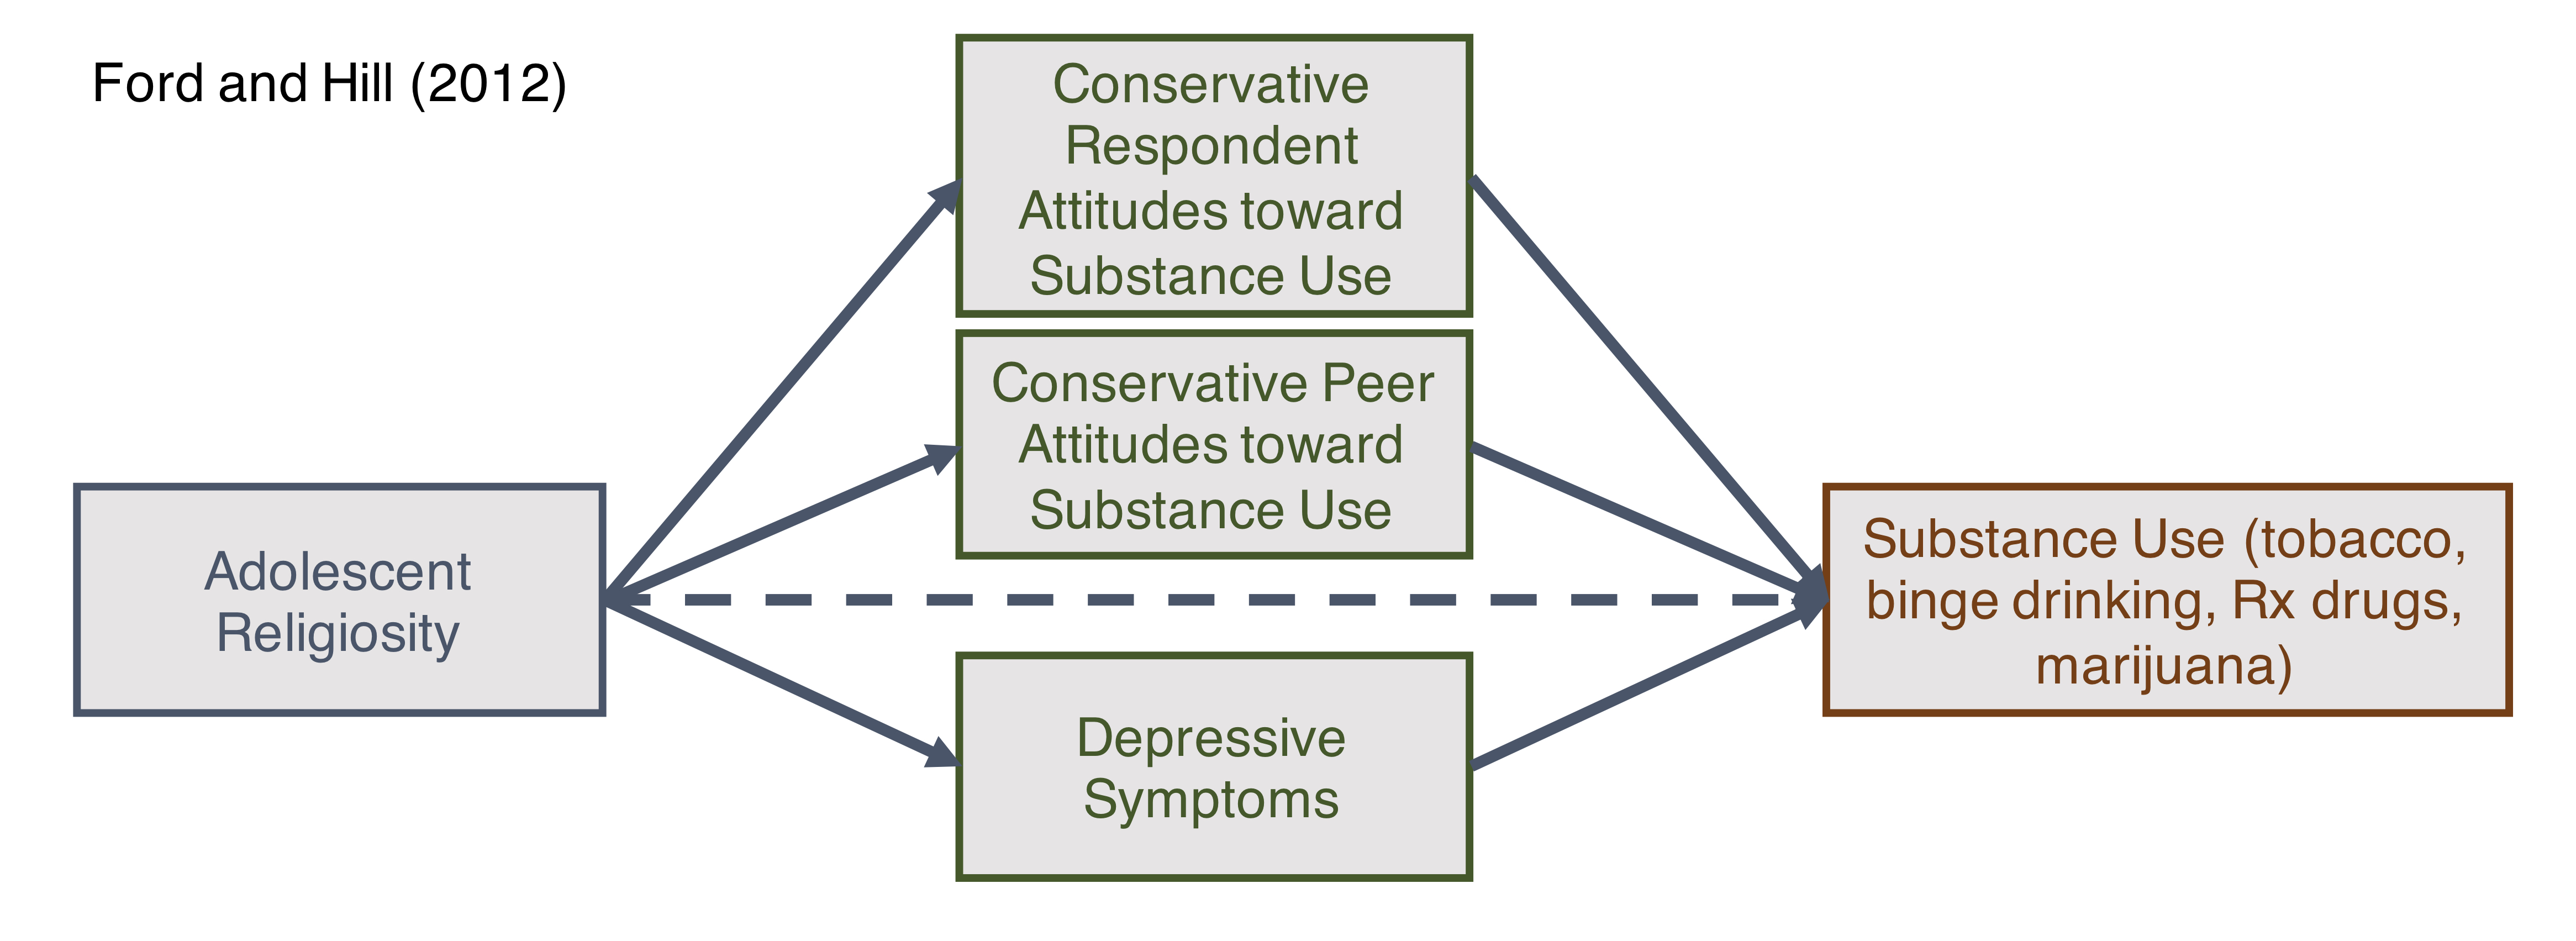
\includegraphics[width=\linewidth]{figures/fig_application_model.jpg}
  \caption{Path diagram of the replicated models from Ford and Hill (2012). The depression mediator and all of the outcomes are categorical.}
  \label{fig:theorymed}
\end{figure}

\subsection{Data}\label{data}

To replicate this study, data from the 2014 (most recent) release of
National Survey on Drug Use and Health {[}NSDUH; @Ford2012{]} were used.
As described by @Ford2012, the NSDUH is ``an ongoing study sponsored by
the U.S. Substance Abuse and Mental Health Services Administration that
dates back to the 1970s'' (page 4) and collects data on drug use of
individuals 12 years and older across the United States. Ford's study
used the 2007 data release while the replication uses the 2014. Several
measures\footnote{Notably, this replication study omits the "heavy drinking" outcome because positive responses to it were very rare in the 2014 data.}
were used to replicate the findings of @Ford2012:

\begin{enumerate}
\def\labelenumi{\arabic{enumi}.}
\tightlist
\item
  Four substance use outcomes (tobacco use, prescription drug use,
  marijuana use, and illicit drug use).
\item
  Religiosity was based on the average response across four items
  relating to church attendance, the importance of religious beliefs to
  the individual, and participation in faith-based activities. Higher
  scores indicated more religiosity.
\item
  Respondent attitudes toward substance use was also the average
  response based on four items gauging the individual's response to
  someone their age using substances. Higher scores indicate more
  conservative attitudes.
\item
  Peer attitudes toward substance use is similar to the respondent
  attitudes except that it was asked how the individual's friends would
  feel about someone their age using substances. Again, the average
  response was used where higher scores indicate more conservative
  attitudes.
\item
  ``Psychological well-being was indicated by major depression,'' (page
  5) which was measured as at least five of the nine possible depression
  symptoms listed in the survey.
\end{enumerate}

\subsubsection{Substance Use}\label{substance-use}

As stated previously, the substance use outcomes are tobacco use,
prescription drug use, marijuana use, and illicit drug use.

\begin{itemize}
\tightlist
\item
  Tobacco use was defined as one of the following three items: 1)
  cigarette use within the last year, 2) smokeless tobacco use within
  the last year, and 3) cigar use within the last year.
\item
  Prescription drug use consisted of four groups of drugs that are being
  used either without a prescription or for the sole purpose of
  obtaining a high within the last year: pain relievers, tranquilizers,
  stimulants, and sedatives.
\item
  Marijuana use was a single item: marijuana use within the last year.
\item
  Illicit drug use was defined as using any of the following drugs
  within the last year: cocaine, crack, heroin, hallucinogens, LSD, PCP,
  ecstasy, inhalants, or meth.
\end{itemize}

\noindent Each outcome was coded as dichotomous: use or no use within
the last year.

\subsubsection{Religiosity}\label{religiosity}

Adolescent religiosity was the mean response across four items: 1) the
number of times attended religious activities in past year, 2) religious
beliefs are important, 3) religious beliefs influence decisions, and 4)
the amount of participation in religious activities. The higher the
average score the more the adolescent is considered to be religious.

\subsubsection{Respondent and Peer
Attitudes}\label{respondent-and-peer-attitudes}

The respondent's conservative views on drug use is the average of four
items, answering the question ``How do you feel about someone your age
using {[}cigarettes daily, marijuana, marijuana monthly, drinking
daily{]}?'' Similarly, the peer's conservative views on drug use is the
average of four items, answering the question ``How do you think your
close friends would feel about you using {[}cigarettes daily, marijuana,
marijuana monthly, drinking daily{]}?''

\subsubsection{Psychological Well-being}\label{psychological-well-being}

Finally, psychological well-being was defined as having had a major
depressive episode in the past year. This was a binary (yes or no)
variable based on ``if they reported experiencing at least five of the
following: felt sad, empty, or depressed most of the day or discouraged;
lost interest or pleasure in most things; experienced changes in
appetite or weight; sleep problems; other noticed you were restless or
lethargic; felt tired or low energy nearly every day; felt worthless
nearly every day; inability to concentrate or make decisions; any
thoughts or plans of suicide,'' {[}@Ford2012, pg. 5{]}.

\subsection{Analyses}\label{analyses}

The mediation analyses were replicated from @Ford2012. Although the
mediation analysis is performed differently herein, the model
specifications were identical to that employed there.

Importantly, @Ford2012 say: ``we use the categorical data method
outlined by MacKinnon (2008) to formally test the indirect effects,''
(pg. 5). This approach uses a significance test based on the estimates
of both \(a\) and \(b\) and their standard errors. However, as stated
throughout this project, the significance alone is insufficient
information to provide for a mediation analysis; effect sizes are also
necessary. Because of this, @Ford2012 continue by discussing the amount
of the association between the predictor and outcome, in percentage
units, that the mediator accounted for. This approach is useful but has
some notable shortcomings. First, depending on the level of
multi-collinearity in the models, the standard errors of the estimates
can be inefficient which reduces the statistical power of this test.
Second, it does not provide the effect size measures that would be most
useful (e.g., the effect a one unit increase in the predictor has on the
outcome through the mediator). Third, the measure is consistently too
conservative with binary outcomes {[}@Jiang2015{]}.

For the replication, then, each of the mediation models reported were
run using MMA in place of the techniques employed by @Ford2012. Four
distinct MMA models, one for each of the substance use outcomes, were
assessed. These were all controlling for (adjusting for) parental
attitudes towards substance use, age, race, sex, and income. The models
included 500 bootstrapped samples to obtain 95\% confidence intervals.

Further, using a variant of the ``difference method,'' the amount of the
total effect that was mediated was calculated using the following: \[
\text{Proportion mediated} =\frac{indirect}{indirect + direct}
\] \noindent Finally, the information provided through the use of MMA
was also compared to that produced in the original
paper.\footnote{All analysis code is available on the Open Science Framework (osf.io/753kc) and in the Appendices of this document.}

\section{Conclusions}\label{conclusions}

Ultimately, the goal of this project is to develop, evaluate and apply a
method that can provide meaningful interpretation in mediation when the
mediator and/or outcome is categorical. Each phase builds on this goal,
as is discussed in the following chapters starting with the presentation
of the results of Phase I and Phase II regarding the theory, software,
and evaluation of MMA.

\singlespacing


\end{document}
